\subsubsection{Máquina de cambios}

    Una máquina de cambios (Figura \ref{fig:cambios_1}) es un mecanismo utilizado para permitir el paso de las formaciones de una vía a una ramificación del recorrido principal. Esto se realiza mediante el movimiento de la aguja del cambio (riel móvil) hacia su respectiva contraaguja (riel fijo) hasta obtener un adecuado acoplamiento que permita la circulación de la formación.

    \begin{figure}[!h]
        \centering
        \includegraphics[width=1\textwidth]{example-image}
        \centering\caption{XXXXX.}
        \label{fig:cambios_1}
    \end{figure}

    En la Figura \ref{fig:cambios_2} se muestra el cambio de vía de la estación Matheu de la Línea Mitre. Se observa que según sea la posición de la máquina de cambios, el tren puede continuar en la misma vía o hacer el cambio a la otra vía.

    \begin{figure}[!h]
        \centering
        \includegraphics[width=1\textwidth]{example-image}
        \centering\caption{XXXXX.}
        \label{fig:cambios_2}
    \end{figure}

    En la Figura \ref{fig:cambios_3} se muestran las posiciones que puede adoptar el cambio. En la posición normal, los trenes pueden circular de forma directa, en paralelo, por la vía principal en sentidos opuestos. En la posición reversa, en cambio, se permite el intercambio de trenes de una rama principal a otra en sentido opuesto o a una ramificación secundaria de la red.

    \begin{figure}[!h]
        \centering
        \includegraphics[width=1\textwidth]{example-image}
        \centering\caption{XXXXX.}
        \label{fig:cambios_3}
    \end{figure}

    Hablar de comando, correspondencia y accion. Figura \ref{fig:cambios_4}

    \lipsum[1]
    
    \begin{figure}[!h]
        \centering
        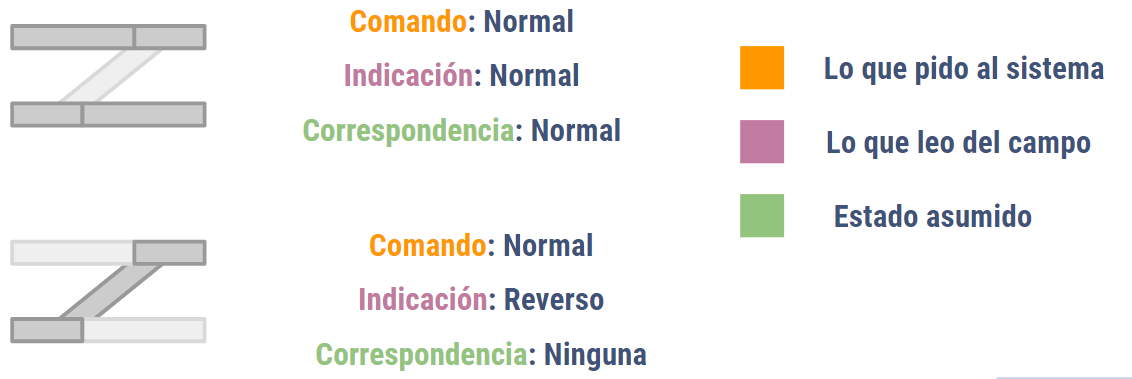
\includegraphics[width=1\textwidth]{Figuras/cambios}
        \centering\caption{XXXXX.}
        \label{fig:cambios_4}
    \end{figure}

EXPLICAR MAS DE CAMBIOS